\section{Эволюционные стратегии}

\subsection{Идея эволюционных стратегий}

Когда мы пытаемся генерировать $k \HM+ 1$-ое поколение, используя особей $k$-го поколения в качестве исходного материала, единственная зависимость от всей истории заложена в составе $k$-ой популяции. Мы можем рассмотреть распределение, из которого появляются особи очередной популяции: весь смысл нашей процедуры отбора в том, чтобы это распределение для очередной итерации поменялось так, что вероятность появления более хороших особей стала выше. Давайте обобщим эту идею: будем в явном виде хранить распределение для порождения особей новой популяции и по информации со всей популяции аккумулировать всю информацию внутри его параметров --- <<скрещивать все особи>>.

\begin{definition}
Распределение $q(\theta \HM\mid \lambda_k)$, из которого генерируются особи $k$-ой популяции, называется \emph{эволюционной стратегией} (evolutionary strategy, ES):
$$\Pop_{k} \coloneqq \{\theta_i \sim q(\theta \HM\mid \lambda_k) \mid i \in \{1, 2 \dots N\} \}$$
где $\lambda_k$ --- параметры эволюционной стратегии.
\end{definition}

\needspace{7\baselineskip}
\begin{wrapfigure}{r}{0.4\textwidth}
\centering
\vspace{-0.6cm}
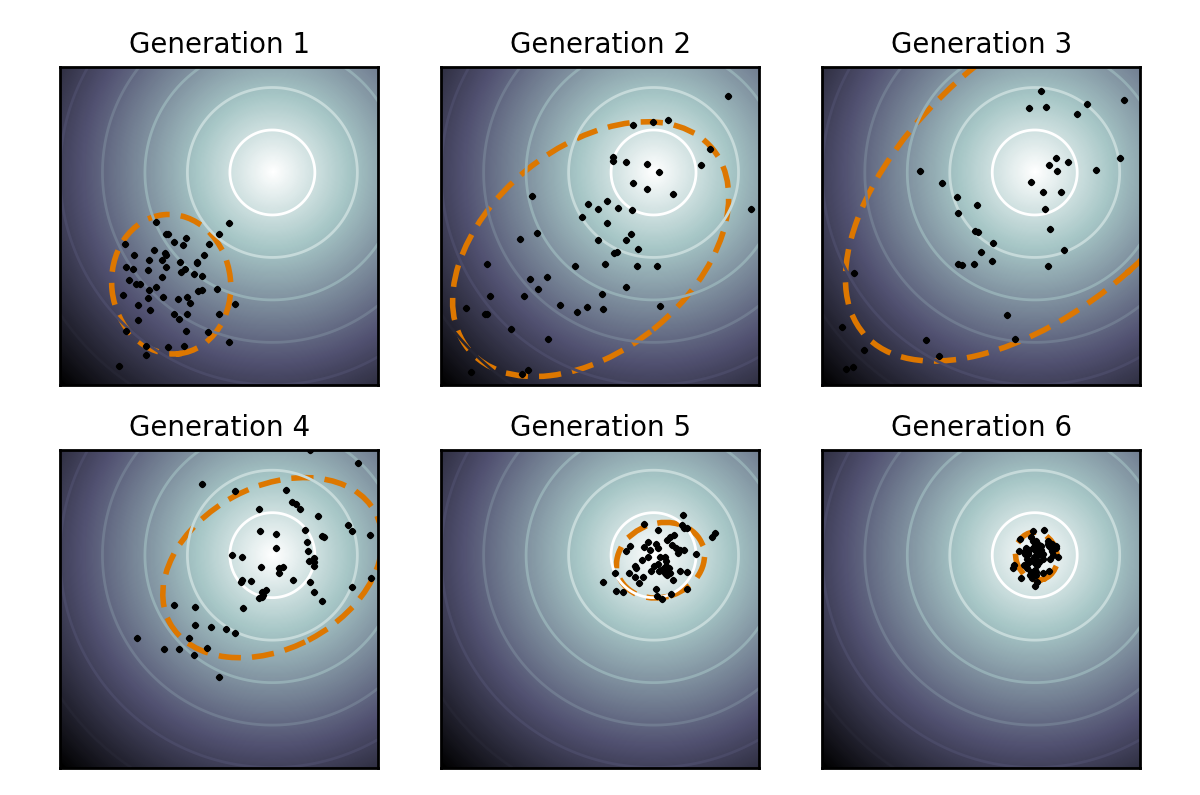
\includegraphics[width=0.4\textwidth]{Images/evolution_strategy.png}
\vspace{-0.5cm}
\end{wrapfigure}

Из каких соображений подбирать $\lambda_k$ на очередном шаге? В принципе, мы хотели бы найти такой генератор особей, что их оценки как можно больше, то есть нащупать область $\Theta$ с высоким значением $J(\theta)$. Эти соображения можно формализовать довольно по-разному и таким образом оправдывать разные мета-эвристики. В частности, мы можем сказать, что $\lambda$ есть особь или несколько особей (что приведёт нас к примерно ранее рассматривавшимся алгоритмам\footnote{понятие эволюционных стратегий довольно общее и размытое --- любой эволюционный алгоритм <<неявно>> определяет распределение для порождения особей очередной популяции и формально подпадает под эволюционные стратегии. Можно считать, что здесь ключевая идея заключается в том, что мы явно ищем это распределение в некотором параметрическом семействе.}), но мы можем отойти от пространства $\Theta$ и учить модель-генератор особей с какой-то хорошей параметризацией $\lambda$. Мы дальше рассмотрим две основные идеи, как это можно делать.

\subsection{Оценка вероятности редкого события}

Первую идею возьмём немного сбоку. Допустим, стоит задача оценки вероятности редкого события:
\begin{equation}\label{rareeventestimation}
l = \Prob(f(x) \ge \gamma) = \E_{x \sim p(x)} \mathbb{I}\left[ f(x) \ge \gamma \right] \,\text{---}\, ?
\end{equation}
где $p(x)$ --- некоторое распределение, $f \colon X \to \R$ --- функционал, $\gamma$ --- некоторый порог. 

Под словами <<редкое событие>> подразумевается, что выражение в индикаторе не равно нулю с вероятностью, крайне близкой к нулю. Это означает, что Монте-Карло оценка с разумным числом сэмплов $N$ выдаст или ноль или $\frac{1}{N}$, если один раз повезёт; короче, лобовой подход не годится.

Хочется сэмплировать $x$ не из того распределения, которое нам дали --- $p(x)$, --- а из чего-нибудь получше. Для этого применим \emph{importance sampling} с некоторым распределением $q(x)$, которое мы будем выбирать сами:
\begin{equation}\label{is_repe}
l = \E_{x \sim q(x)} \frac{p(x)}{q(x)} \mathbb{I}\left[ f(x) \ge \gamma \right]
\end{equation}

Нам хочется выбрать такое $q(x)$, чтобы дисперсия Монте-Карло оценки такого интеграла была как можно меньше. Желание может быть исполнено:
\begin{proposition}
Дисперсия Монте-Карло оценки \eqref{is_repe} минимальна при 
\begin{equation}\label{optimal_q_is_repe}
q(x) \propto p(x)\mathbb{I}\left[ f(x) \ge \gamma \right]
\end{equation}

\begin{proof}
Искомое значение $l$ \eqref{rareeventestimation} является нормировочной константой такого распределения. Подставим данное $q(x)$ в подынтегральную функцию:
$$
\frac{p(x)}{q(x)} \mathbb{I}\left[ f(x) \ge \gamma \right] = l \frac{p(x)\mathbb{I}\left[ f(x) \ge \gamma \right]}{p(x)\mathbb{I}\left[ f(x) \ge \gamma \right]} = l
$$
Поскольку всё сократилось, для любых сэмплов $x \sim q(x)$ значение Монте-Карло оценки будет равно $l$; то есть, дисперсия равна нулю.
\end{proof}
\end{proposition}

Посчитать такое $q(x)$ мы не можем, однако можем пытаться приблизить в параметрическом семействе $q(x \HM\mid \lambda)$, минимизируя, например, такую KL-дивергенцию:
$$\KL(q(x) \parallel q(x \mid \lambda)) = \const(\lambda) - \E_{q(x)} \log q(x \mid \lambda) \to \min_\lambda$$
Единственное зависящее от параметров $\lambda$ слагаемое называется \emph{кросс-энтропией} (cross entropy) и даёт название методу.

Пока что мы променяли шило на мыло, поскольку для такой оптимизации всё равно нужно уметь сэмплировать из $q(x)$. Однако от задачи оценки числа (которую мы кроме как через Монте-Карло особо решать не умеем) мы перешли к поиску распределения. Поскольку это распределение мы строили так, чтобы оно помогало сэмплировать нам точки из редкого события, можно воспользоваться им же с прошлой итерации, чтобы помочь самим себе решать ту же задачу лучше. А то есть: строим последовательность $q(x \HM\mid \lambda_k)$, $\lambda_0$ --- любое, на очередной итерации:
\begin{align*}
\lambda_{k+1} &= \argmin_{\lambda} -\E_{q(x)} \log q(x \mid \lambda) = \\
\{\text{подставляем вид оптимального $q(x)$ из \eqref{optimal_q_is_repe}}\} &= \argmin_{\lambda} -\E_{p(x)} \mathbb{I}\left[ f(x) \ge \gamma \right] \log q(x \mid \lambda) = \\
\{\text{importance sampling через $q(x \mid \lambda_{k})$}\} &= \argmin_{\lambda} -\E_{q(x \mid \lambda_{k})} \frac{p(x)}{q(x \mid \lambda_{k})}\mathbb{I}\left[ f(x) \ge \gamma \right] \log q(x \mid \lambda)
\end{align*}

Каждая задача нахождения $\lambda_k$ всё ещё тяжела в связи с тем, что подынтегральное выражение всё ещё почти всегда ноль. Ключевая идея: поскольку мы теперь строим целую последовательность, мы можем поначалу решать сильно более простую задачу, разогревая $\gamma$. Будем на $k$-ом шаге брать $\gamma$ не из условия задачи, а поменьше, так, чтобы с итерациями $\gamma$ увеличивалась (и мы решали бы задачу, всё более похожую на ту, что требовалось решить исходно), и одновременно достаточное число сэмплов значения подынтегральной функции были отличны от нуля.

Важно, что мы можем не задавать заранее последовательность $\gamma_k$, а определять очередное значение прямо на ходу, например, исходя из сэмплов $x_1 \dots x_N \sim q(x \mid \lambda_{k})$ и значений $f(x)$ в них.

\begin{algorithm}[label=alg:rareeventestimate]{Метод Кросс-Энтропии для оценки вероятности редкого события}
\textbf{Вход:} распределение $p(x)$, функция $f(x)$, порог $\gamma$ \\
\textbf{Гиперпараметры:} $q(x \mid \lambda)$ --- параметрическое семейство, $N$ --- число сэмплов, $M$ --- порог отбора

\vspace{0.3cm}
Инициализируем $\lambda_0$ произвольно. \\
\textbf{На $k$-ом шаге:}
\begin{enumerate}
    \item сэмплируем $x_1 \dots x_N \sim q(x \mid \lambda_k)$
    \item сортируем значения $f(x_i)$: $f_{(1)} \le f_{(2)} \le \dots \le f_{(N)}$
    \item полагаем $\gamma_k \coloneqq \min(\gamma, f_{(M)})$
    \item решаем задачу оптимизации:
    \begin{equation}\label{CEM_optimization_general}
    \lambda_{k+1} \leftarrow \argmax_{\lambda} \frac{1}{N} \sum_{j=1}^N \mathbb{I}[f(x_j) \ge \gamma_k]\frac{p(x_j)}{q(x_j \mid \lambda_k)} \log q(x_j \mid \lambda)
    \end{equation}
    \item \textbf{критерий останова:} $\gamma_k = \gamma$
\end{enumerate}

\textbf{Получение итоговой оценки:}
\begin{enumerate}
    \item сэмплируем $x_1 \dots x_N \sim q(x \mid \lambda_k)$
    \item возвращаем
    $$l \approx \frac{1}{N} \sum_{j=1}^N \mathbb{I}[f(x_j) \ge \gamma_k]\frac{p(x_j)}{q(x_j \mid \lambda_k)}$$
\end{enumerate}
\end{algorithm}

\subsection{Метод Кросс-Энтропии для стохастической оптимизации}

Ну, в рассуждении было видно, что мы практически учим $q(x \mid \lambda)$ нащупывать область с высоким значением заданной функции без использования какой-либо информации о ней. Поэтому мы можем адаптировать метод, чтобы он стал мета-эвристикой. Для этого вернёмся к нашей задаче безградиентной оптимизации:
$$J(\theta) \to \max_{\theta}$$
и перепишем алгоритм \ref{alg:rareeventestimate} в условиях, когда порог $\gamma$ <<не ограничен>>, ну или что тоже самое, $\gamma \HM\coloneqq \max\limits_{\theta} J(\theta)$. Формально мы также можем выбирать любое $p(x)$; положим $p(x) \coloneqq q(x \mid \lambda_k)$, просто чтобы в задаче \eqref{CEM_optimization_general} сократилась importance sampling коррекция. Мы получим очень простой на вид алгоритм, в котором фактически на очередном шаге минимизируется такое расстояние:
$$\KL(\mathbb{I}[J(x) \ge \gamma_k] q(x \mid \lambda_{k-1}) \parallel q(x \mid \lambda_k)) \to \min_{\lambda_k},$$
где первое распределение задано с точностью до нормировочной константы.

\begin{algorithm}{Метод Кросс-Энтропии для оптимизации с оракулом нулевого порядка}
\textbf{Вход:} оракул $\hat{J}(\theta)$ \\
\textbf{Гиперпараметры:} $q(\theta \mid \lambda)$ --- параметрическое семейство, $N$ --- число сэмплов, $M$ --- порог отбора

\vspace{0.3cm}
Инициализируем $\lambda_0$ произвольно. \\
\textbf{На $k$-ом шаге:}
\begin{enumerate}
    \item сэмплируем $\Pop_k \coloneqq \left( \theta_i \sim q(\theta \mid \lambda_k) \mid i \in \{1, 2, \dots, N\} \right)$
    \item проводим отбор $\Pop^{+}_k \coloneqq \Seltop_M(\Pop_k)$
    \item решаем задачу оптимизации:
    $$\lambda_{k+1} \leftarrow \argmax_{\lambda} \sum_{\theta \in \Pop^{+}_k} \log q(\theta \mid \lambda)$$
\end{enumerate}
\end{algorithm}

Видно, что мы по сути действуем эволюционно: хотим генерировать при помощи распределения $q$ точки из области, где значение функции велико; берём и сэмплируем несколько точек из текущего приближения; из сгенерированных отбираем те, где значение функции было наибольшим и учим методом максимального правдоподобия повторять эти точки. Поскольку некоторая доля плохих точек было выкинуто из выборки, распределение, которое учит очередное $q(x \mid \lambda_k)$, лучше предыдущего. Это первый способ обучения эволюционных стратегий.

\subsection{Метод Кросс-Энтропии для обучения с подкреплением (CEM)}

В обучении с подкреплением в кросс-энтропийном методе можно сделать ещё один очень интересный шаг. В отличие от всех остальных рассматриваемых в этой главе мета-эвристик, мы можем проводить эволюционный отбор не в пространстве возможных стратегий (в пространстве $\Theta$), а в пространстве траекторий. У нас будет одна текущая стратегия, из которой мы сгенерируем несколько траекторий, и в силу стохастичности некоторые из этих траекторий выдадут лучший результат, чем другие. Мы отберём лучшие и будем методом максимального правдоподобия (по сути, имитационным обучением) учиться повторять действия из лучших траекторий.  

\begin{algorithm}{Cross Entropy Method}
\textbf{Гиперпараметры:} $\pi(a \mid s, \theta)$ --- стратегия с параметрами $\theta$, $N$ --- число сэмплов, $M$ --- порог отбора

\vspace{0.3cm}
Инициализируем $\theta_0$ произвольно. \\
\textbf{На $k$-ом шаге:}
\begin{enumerate}
    \item сэмплируем $N$ траекторий $\Traj_1 \dots \Traj_N$ игр при помощи стратегии $\pi(a \mid s, \theta_k)$
    \item считаем кумулятивные награды $R(\Traj_i)$
    \item сортируем значения: $R_{(1)} \le R_{(2)} \le \dots \le R_{(N)}$
    \item полагаем $\gamma_k \coloneqq R_{(M)}$
    \item решаем задачу оптимизации:
    $$\theta_{k+1} \leftarrow \argmax_{\theta} \frac{1}{N} \sum_{j=1}^N \mathbb{I}[R(\Traj_j) \ge \gamma_k] \sum_{s, a \in \Traj_j} \log \pi(a \mid s, \theta)$$
\end{enumerate}
\end{algorithm}

% TODO: примеры, схожесть с ML-оценкой.

\subsection{Натуральные эволюционные стратегии (NES)}\label{subsec:nes}

Рассмотрим альтернативный вариант\footnote{смысл названия <<натуральные эволюционные стратегии>> (natural evolution strategies) будет объяснён позже.} подбора параметров эволюционной стратегии $q(\theta \mid \lambda)$. Будем подбирать $\lambda$, исходя из следующего функционала:
\begin{equation}\label{es}
g(\lambda) \coloneqq \E_{\theta \sim q(\theta \mid \lambda)} J(\theta) \to \max_{\lambda}
\end{equation}

Будем оптимизировать этот функционал градиентно по $\lambda$. Давайте подробно разберём, как дифференцировать функции подобного вида, поскольку в дальнейшем мы будем активно пользоваться этой техникой.

\begin{theorem}
\begin{equation}\label{ESgradient}
    \nabla_\lambda g(\lambda) = \E_{\theta \sim q(\theta \mid \lambda)} \nabla_\lambda \log q(\theta \mid \lambda) J(\theta)
\end{equation}
\beginproof
\begin{align*}
\nabla_\lambda g(\lambda) &= \nabla_\lambda \E_{\theta \sim q(\theta \mid \lambda)} J(\theta) = \\
= \{ \text{мат.ожидание --- это интеграл} \} &= 
\nabla_\lambda \int\limits_\Theta q(\theta \mid \lambda)J(\theta) \diff \theta = \\
= \{ \text{проносим градиент внутрь интеграла} \} &=
\int\limits_\Theta \nabla_\lambda q(\theta \mid \lambda)J(\theta) \diff \theta = (*)
\end{align*}

Теперь мы применим стандартный технический трюк, называемый \emph{log-derivative trick}: мы хотим преобразовать данное выражение к виду мат.ожидания по $q(\theta \mid \lambda)$ от чего-то. Как мы сейчас увидим, это <<что-то>> --- градиент логарифма правдодобия. Мы воспользуемся следующим тождеством:
\begin{equation}\label{logderivtrick}
\nabla_\lambda \log q(\theta \mid \lambda) = \frac{\nabla_\lambda q(\theta \mid \lambda)}{q(\theta \mid \lambda)}
\end{equation}

Домножим и поделим наше выражение на $q(\theta \mid \lambda)$, чтобы получить внутри интеграла мат.ожидание:
\begin{align*}
(*) &= \int\limits_\Theta q(\theta \mid \lambda) \frac{\nabla_\lambda q(\theta \mid \lambda)}{q(\theta \mid \lambda)} J(\theta) \diff \theta = \\
= \{ \text{замечаем градиент логарифма \eqref{logderivtrick} } \}
&= \int\limits_\Theta q(\theta \mid \lambda) \nabla_\lambda \log q(\theta \mid \lambda) J(\theta) \diff \theta = \\
= \{ \text{выделяем мат.ожидание} \}
&= \E_{\theta \sim q(\theta \mid \lambda)} \nabla_\lambda \log q(\theta \mid \lambda) J(\theta) \tagqed
\end{align*}

%\footnotetext{здесь нужно требовать некоторые минимальные условия регулярности, см., например, \href{https://www.colorado.edu/amath/sites/default/files/attached-files/billingsley.pdf}{теорему 16.8 книги Биллингсли (стр.~212)}: достаточным условием является измеримость, интегрируемость и ограниченность $J(\theta)$ на $\Theta$.}
\end{theorem}

Итак, есть следующая идея: сгенерируем популяцию $\Pop_k$ при помощи $q(\theta \mid \lambda_k)$, после чего воспользуемся особями как сэмплами для несмещённой оценки градиента функционала \eqref{es}, чтобы улучшить параметры $\lambda$ и впоследствии сгенерировать следующее поколение $\Pop_{k+1}$ из более хорошего распределения.

% \begin{algorithm}[label=nes]{Естественная эволюционная стратегия}
% \textbf{Дано:} оракул $\hat{J}(\theta)$ \\
% \textbf{Гиперпараметры:} $q(\theta \mid \lambda)$ --- эволюционная стратегия, $N$ --- размер популяции, SGD оптимизатор

% \vspace{0.3cm}
% Инициализируем $\lambda$ случайно. \\
% \textbf{На $k$-ом шаге:}
% \begin{enumerate}
%     \item генерируем популяцию: $\Pop_{k} \coloneqq \{\theta_i \sim q(\theta \HM\mid \lambda) \mid i \in \{1, 2 \dots N\} \}$
%     \item проводим оценивание градиента: $\nabla \coloneqq \frac{1}{N} \sum\limits_{\theta \in \Pop_k} \nabla_\lambda \log q(\theta \mid \lambda) \hat{J}(\theta)$
%     \item делаем шаг градиентного подъёма по $\lambda$, используя $\nabla$. 
% \end{enumerate}
% \end{algorithm}

\subsection{OpenAI-ES}

Рассмотрим подход на примере OpenAI-ES, где рассматривается обучение нейросети (с фиксированной топологией) с вещественными весами $\Theta \equiv \R^h$, и полагается
\begin{equation}\label{openai_es}
q(\theta \mid \lambda) \coloneqq \N(\lambda, \sigma^2I_{h \times h})
\end{equation}
где $\sigma$ --- гиперпараметр, $\lambda \in \R^h$ --- по сути, кодирует одну особь, $I_{h \times h}$ --- диагональная единичная матрица размера $h \times h$.

\begin{theorem}
Для эволюционной стратегии \eqref{openai_es} оценка градиента \eqref{es} равна
\begin{equation}\label{openai_es_gradient}
\nabla_\lambda g(\lambda) = \frac{1}{N\sigma^2} \sum_{\theta \in \Pop} \hat{J}(\theta) (\theta - \lambda)
\end{equation}
\begin{proof}
$$\nabla_\lambda \log q(\theta \mid \lambda) = -\nabla_\lambda \frac{\left(\theta - \lambda \right)^T \left( \theta - \lambda \right)}{2 \sigma^2} = \frac{\theta - \lambda}{\sigma^2}$$
Достаточно подставить выражение в общую формулу \eqref{ESgradient}.
\end{proof}
\end{theorem}

Полученная формула легко интерпретируема: мы находимся в некотором <<центре>> $\lambda$, который является нашим <<текущим найденным решением>>. Дальше мы сэмплируем несколько векторов $\theta - \lambda$ из стандартного нормального распределения и складываем эти вектора (<<скрещиваем всех детей>>) с весами, пропорциональными приспособленности.

% \begin{remark}
% Последним изменением является введение в процедуру жадного отбора: оценки среднего и ковариации проходят только по особям $\Pop_k^{+}$ с наибольшей приспособленностью. Также применяется rank-based shaping...
% \end{remark}

\begin{remark}
Подход работает при большом количестве серверов и ещё одном трюке, позволяющем не обмениваться векторами $\theta$ (имеющими размерность, например, по числу параметров нейросети) между процессами. Для этого достаточно зафиксировать random seed на всех процессорах, в каждом процессе генерировать всё поколение, оценивать только особь с соответствующим процессу номеру и обмениваться с другими процессами исключительно оценками $\hat{J}$ (скалярами!). Цель такой процедуры --- избежать обмена весами нейросетей (пусть даже не очень больших) между серверами. За счёт параллелизации удаётся так <<обучать>> сетки играть в одну игру Атари за 10 минут. Если у вас есть 1440 процессоров. Естественно, ни про какой sample efficiency речь не идёт. 
\end{remark}

\begin{example}[OpenAI-ES]
\begin{center}
\animategraphics[controls, width=\linewidth]{1}{Images/ES/es-}{0}{5}
\end{center}
\end{example}

Рассмотрим альтернативный взгляд на этот алгоритм. Допустим, мы находимся в точке $\theta$ и хотим сдвинуться как бы по градиенту $J(\theta)$, который вычислить мы не можем. Но мы можем приблизить градиент вдоль любого направления $\nu$, например, так:
$$ \left. \nabla \right|_{\nu} J(\theta) \approx \frac{\hat{J}(\theta + \sigma \nu) - \hat{J}(\theta)}{\sigma}$$
для некоторого небольшого скаляра $\sigma$.

Лобовая идея\footnote{в алгоритме ARS (Advanced Random Search, хотя такой подход не совсем <<случайный поиск>>) делается ровно это, за тем небольшим исключением, что используется приближение градиента по направлению за два вызова оракула:
$$ \left. \nabla \right|_{\nu} J(\theta) \approx \frac{\hat{J}(\theta + \sigma \nu) - \hat{J}(\theta - \sigma \nu)}{2\sigma}$$}: давайте возьмём $N$ случайных направлений $\nu_1 \dots \nu_N \sim \N(0, I)$ и сделаем шаг по всем этим направлениям:
\begin{equation}\label{ars}
\theta_{k+1} \coloneqq \theta_k + \alpha \underbrace{\sum_{i=0}^N \frac{\hat{J}(\theta + \sigma \nu_i) - \hat{J}(\theta)}{\sigma}\nu_i}_{\text{приближение градиента}}
\end{equation}
где $\alpha$ --- learning rate.

\begin{proposition}
Формулы \eqref{ars} и \eqref{openai_es_gradient} эквивалентны.
\begin{proof}
Поскольку $\nu$ сэмплируется из стандартной гауссианы, то в среднем:
$$\E_{\nu \sim \N(0, I)} \frac{\hat{J}(\theta)}{\sigma} \nu = \frac{\hat{J}(\theta)}{\sigma} \E_{\nu \sim \N(0, I)} \nu = 0$$
Следовательно, \eqref{ars} оценивает тот же градиент, что и формула
$$\theta_{k+1} \coloneqq \theta_k + \alpha \sum_{i=0}^N \frac{\hat{J}(\theta + \sigma \nu_i)}{\sigma}\nu_i,$$
что совпадает с формулой OpenAI-ES с точностью до замены обозначений: достаточно заметить, что $\theta + \sigma \nu$ есть сэмпл из $\N(\theta, \sigma^2 I)$.
\end{proof}
\end{proposition}

\subsection{Адаптация матрицы ковариации (CMA-ES)}

Более глубокомысленно было бы для $\Theta \equiv \R^{h}$ адаптировать не только среднее, но и матрицу ковариации, которая имеет смысл <<разброса>> очередной популяции. Covariance Matrix Adaptation Evolution Strategy (CMA-ES) --- алгоритм, включающий довольной большой набор эвристик, в основе которого лежит эволюционная стратегия, адаптирующая не только среднее, но и матрицу ковариации:
\begin{equation}\label{covadapt}
q(\theta \mid \lambda) \coloneqq \N(\mu, \Sigma)
\end{equation}
где $\lambda \coloneqq (\mu, \Sigma)$.

\begin{remark}
Нам придётся хранить матрицу ковариации размера $\R^{h \times h}$, где $h$ --- количество параметров нашей стратегии ($\Theta \HM\equiv \R^h$). Если стратегия задана нейронной сетью, то, чтобы такое было возможно, сеть должна быть по современным меркам минимальнейшей. Однако, во многих задачах непрерывного управления это довольно типичная ситуация, когда на вход в качестве состояния подаётся небольшой (размера 100-200) вектор, а на выходе также ожидается вектор размера порядка 10-30. Тогда стратегия может быть задана полносвязной нейросетью всего в несколько слоёв, и хранить $\Sigma$ теоретически становится возможно. 
\end{remark}

Мы рассмотрим только основную часть формул алгоритма, касающихся формулы обновления $\Sigma$. Посмотрим на формулу для обновления среднего \eqref{openai_es_gradient} (с точностью до learning rate):
\begin{equation}\label{cmaes_mu_update}
\mu_{k+1} = \mu_k + \alpha\sum_{\theta \in \Pop_k} \underbrace{\hat{J}(\theta)}_{\text{вес}} \underbrace{\left( \theta - \mu_k \right)}_{\text{\shortstack{<<предлагаемое>> \\ особью изменение}}}
\end{equation}

Для обновления матрицы ковариации будем рассуждать также: каждая особь популяции $\theta$ <<указывает>> на некоторую ковариацию $\left( \theta - \mu_k \right)\left( \theta - \mu_k \right)^T$ и таким образом <<предлагает>> следующее изменение:
$$\left( \theta - \mu_k \right)\left( \theta - \mu_k \right)^T - \Sigma_k,$$
где $\Sigma_k$ --- матрица ковариации на текущей итерации. Усредним эти <<предложения изменения>> по имеющейся популяции, взвесив их на $\hat{J}(\theta)$, и получим <<градиент>> для обновления матрицы:
\begin{equation}\label{cmaes_sigma_update}
\Sigma_{k+1} \coloneqq \Sigma_k + \alpha \sum_{\theta \in \Pop_k} \hat{J}(\theta) \left( \left( \theta - \mu_k \right)\left( \theta - \mu_k \right)^T - \Sigma_k \right)
\end{equation}

Здесь нужно оговориться, что мы используем оценку ковариации как бы <<методом максимального правдоподобия при условии известного среднего $\mu_k$>> (мы знаем, что именно с таким средним генерировались особи прошлой популяции)\footnote{мы бы пришли к немного другим формулам, если бы использовали метод максимального правдоподобия при условии неизвестного среднего ($\mu_k$ заменилось бы на $\mu_{k+1}$):
$$\left( \theta - \mu_{k+1} \right)\left( \theta - \mu_{k+1} \right)^T - \Sigma_k$$}. Исторически к этим формулам пришли эвристически, но позже у формулы появилось теоретическое обоснование.

\begin{theorem}
Формулы \eqref{cmaes_mu_update} и \eqref{cmaes_sigma_update} для обновления $\lambda = (\mu, \Sigma)$ являются формулами натурального градиентного спуска для \eqref{es}.
\begin{proof}[Доказательство требует обсуждения такой большой темы, как натуральный градиентный спуск (см. приложение \ref{appendix:ng}), а вывод формулы потребует небольшого введения в Кронекерову алгебру, поэтому доказательство вынесено в приложение \ref{appendix:cmaes}] 
\end{proof}
\end{theorem}

Именно поэтому данный вид алгоритмов для обучения эволюционных стратегий называется <<\emph{натуральными}>> (natural): считается, что функционал \eqref{es} корректнее оптимизировать именно при помощи натурального градиентного спуска, инвариантного к параметризации $q(\theta \mid \lambda)$, а не обычного.

\begin{example}[CMA-ES (упрощ.)]
\needspace{10\baselineskip}
\begin{center}
\animategraphics[controls, width=\linewidth]{1}{Images/CMA_ES/cma_es-}{0}{9}
\end{center}
\end{example}

\begin{example}
Эволюционные стратегии и особенно CMA-ES весьма успешно применимы в задачах непрерывного управления вроде Locomotion (пример \ref{ex:locomotion}), в которых нужно научить разных существ ходить. Много интересных примеров можно найти в \href{https://www.youtube.com/watch?v=pgaEE27nsQw}{этом видео}.
\end{example}

Если мы попробуем проделать с данным подходом (оптимизацией \eqref{es}) проделать тот же трюк, что и с кросс-энтропийным методом, и попытаемся считать градиент <<в пространстве траекторий>>, а не в пространстве стратегий, то получим методы оптимизации $J(\theta)$ уже первого порядка --- <<policy gradient>> методы. К ним мы перейдём в главе \ref{policygradientchapter}.